
Connectivity is important but sometimes it is not enough and we want some 
robust connectivity. So we introduce \textbf{Bi-connectivity}.
\subsection{Definitions}
\subsubsection{Bi-connectivity}
\begin{itemize}
\item A graph is called biconnected if the removal of any one vertex leaves it 
connected.
\item A graph is called k-connected if the removal of any $k-1$ vertices leaves 
it connected.
\end{itemize}
Examples of connected graph which is not bi-connected.
\begin{figure}[H]
\centering
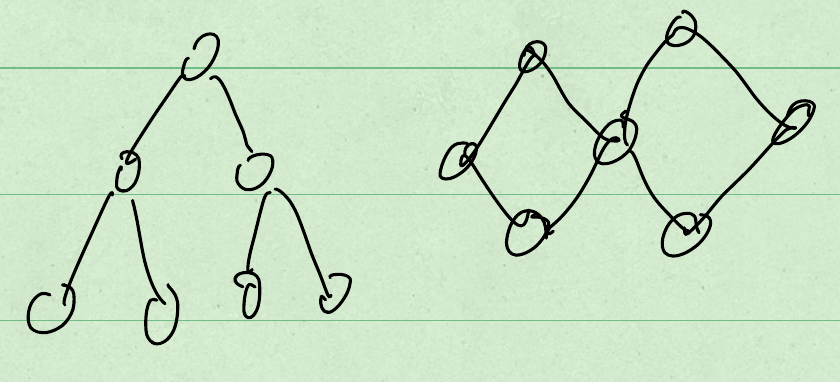
\includegraphics[width=0.5\textwidth]{bi-connectivity.png}
\end{figure}
\subsubsection{Articulation Point}
A vertex in an undirected connected graph is an \textbf{articulation point} (or 
cut vertex) \textbf{iff} removing it (and edges through it) disconnects the 
graph. 

Articulation points represent vulnerabilities in a connected 
network-single points whose failure would split the network into 2 or more 
disconnected components.

\subsubsection{Bi-connected Components}
Bi-connected Components are maximal pieces of the graph that are bi-connected.

\subsubsection{Vertex-disjoint Path}
Two paths are vertex-independent (alternatively, internally 
\textbf{vertex-disjoint}) if they do not have any internal vertex in common. 

Similarly, two paths are edge-independent (or edge-disjoint) if they do not 
have any internal edge in common. Two internally vertex-disjoint paths 
are edge-disjoint, but the converse is not necessarily true.

\subsubsection{Relations on edges}
How to define the relation between two vertices?

\paragraph{Proposal:} If there are two vertex-disjoint paths between $u$ and 
$v$, then $(u, v) \in R$. See example (a) in the following graph.

The proposal does not work because the relation is not Transitive. In other 
words, if $(u, v) \in R$ and $(v, w) \in R$ it is not always the case that 
$(u, w) \in R$.
See example (b) in the following graph. $(1, 6) \in R$ is a false statement.

\begin{figure}[H]
\centering
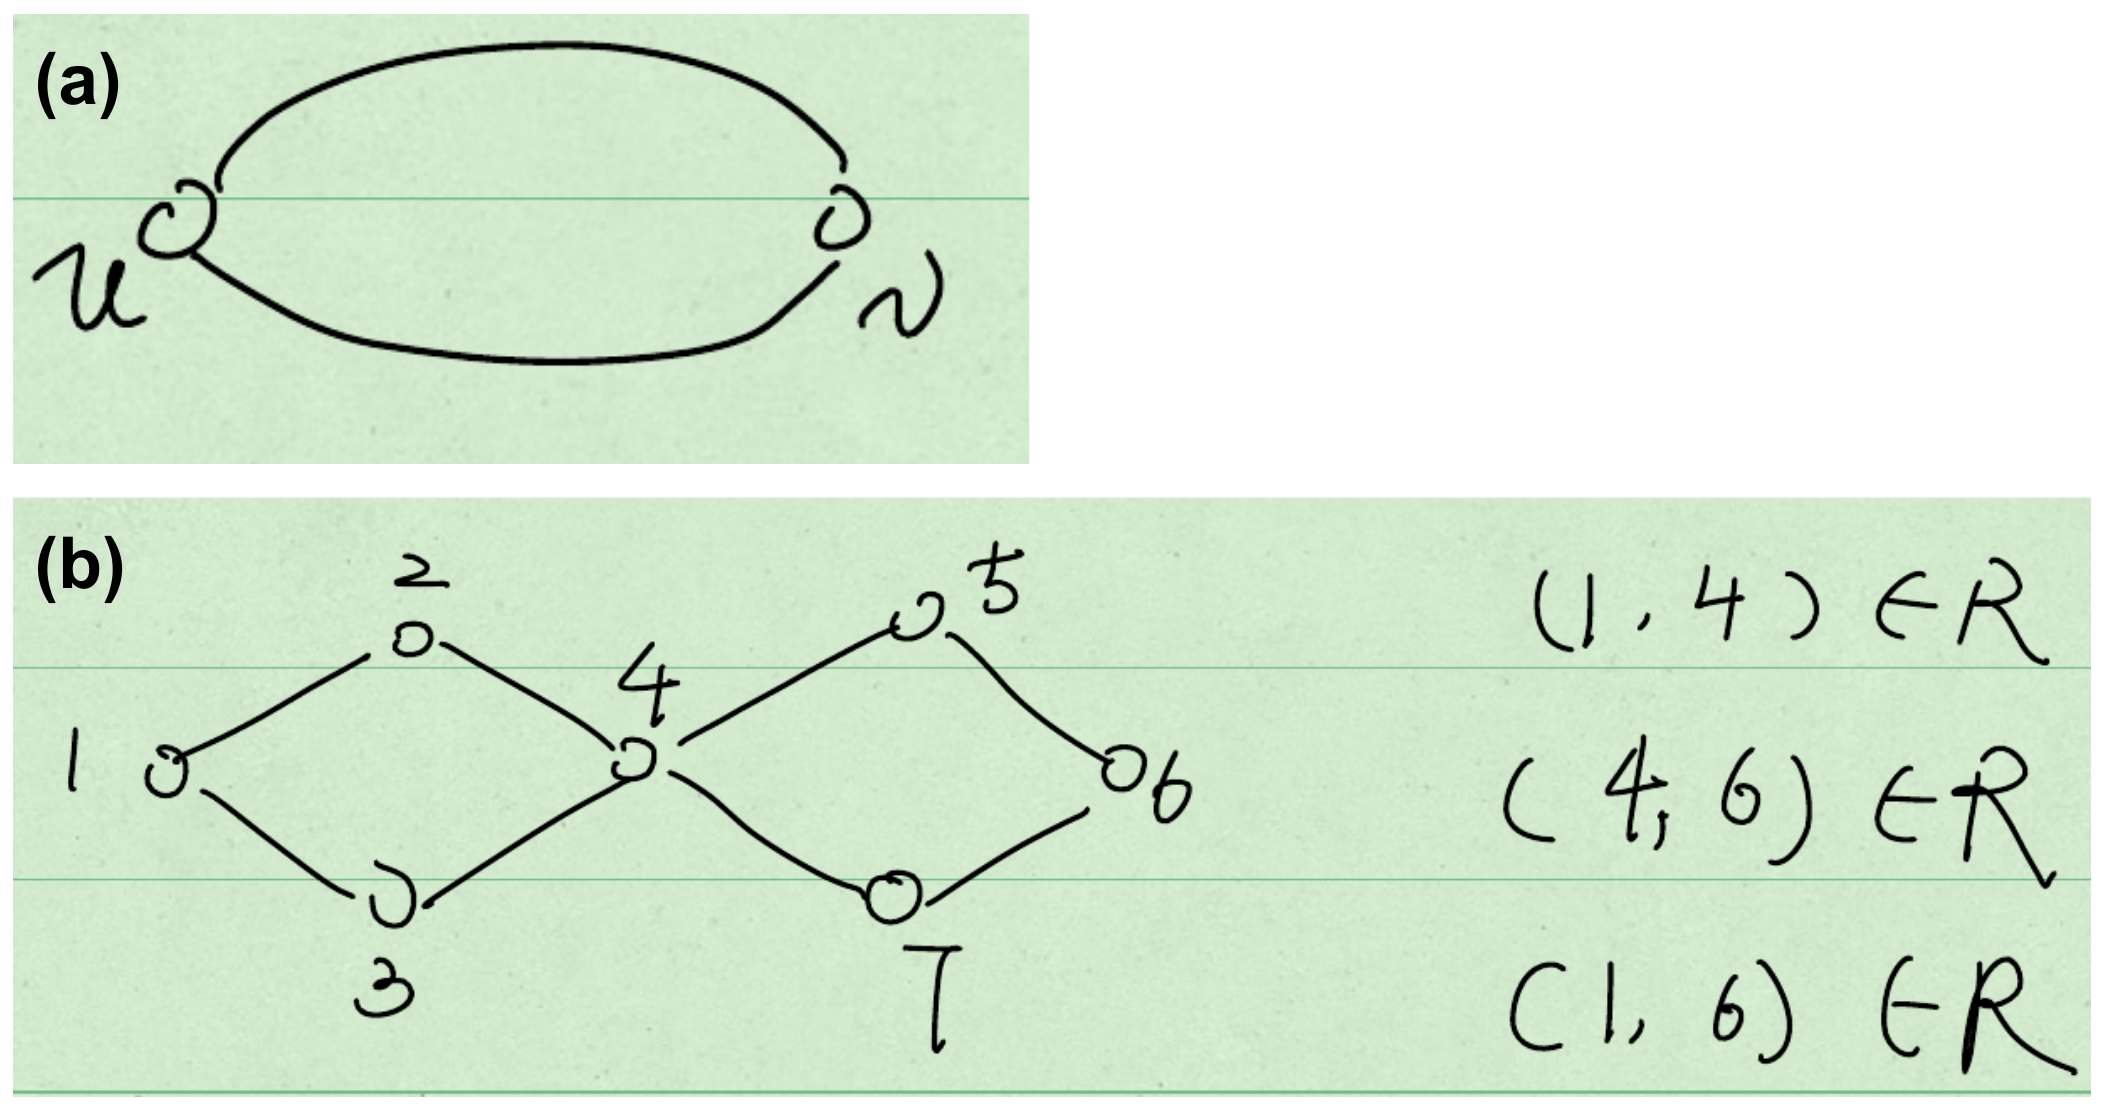
\includegraphics[width=0.5\textwidth]{relation.png}
\end{figure}

\paragraph{The relation $R$ on edges defined as follows:}
\begin{itemize}
\item For any edge $e$, $(e,e) \in R$.
\item If $e_1, e_2$ are two distinct edges, then $(e_1, e_2) \in R$ iff there 
is a simple cycle that passes through $e_1, e_2$.
\end{itemize}

Assume $R$ is an equivalent relation on edges. The property of equivalent 
relation is it divides the set on which it is defined into partitions of 
equivalent class.

Assume $R$ is an equivalence relation on edges. R partitions edges into 
equivalence class $E_1, E_2, \cdots, E_k$. 

For a sanity check, if $k = 1$ then the graph is a bi-connected graph. 
% TODO: ? why
Define component $G_i$ as the graph consist of edges $E_i$ together with a 
vertex set $V_i$ consist of the every point of $E_i$.

A vertex belongs to more than one components iff it is not clean.

\subsection{Find Articulation Points}
Assume $G$ is connected and undirected, start DFS at node $s$, so $s$ is the root of DFS tree.

\subsubsection{Check root of DFS Tree}
\paragraph{Case 1:} Suppose $s$ has one child in DFS tree. In this case, $s$ is 
not an articulation point since the removal of $s$ won't disconnect the graph. 
See example in (a).

\paragraph{Case 2:} Suppose $s$ has more than 1 child in DFS tree. $s$ is 
an articulation point because back edges only go between ancestor and 
descendant. The nodes in subtree $T(v_1)$ and $T(v_2)$ are not ancestor nor 
descendant between each other. Therefore all the paths connecting $T(v_1)$ and $T(v_2)$ must go through $s$. Hence $s$ is an articulation point. See example in (b).

\subsubsection{Check Interior Nodes}

Note that no leaf can be articulation point because moving a leaf the DFS tree is still connected.

Assume $v$ is an internal node and has $k$ leaves. What are the conditions for $v$ to be an articulation point? 
\begin{claim}
 An internal node $v$ is an articulation point \textbf{iff} it has a child $u_i$ such that here is no back edge from the subtree rooted at $u_i$ to a proper ancestor of $v$. See example in (c).
\end{claim}

\begin{figure}[H]
\centering
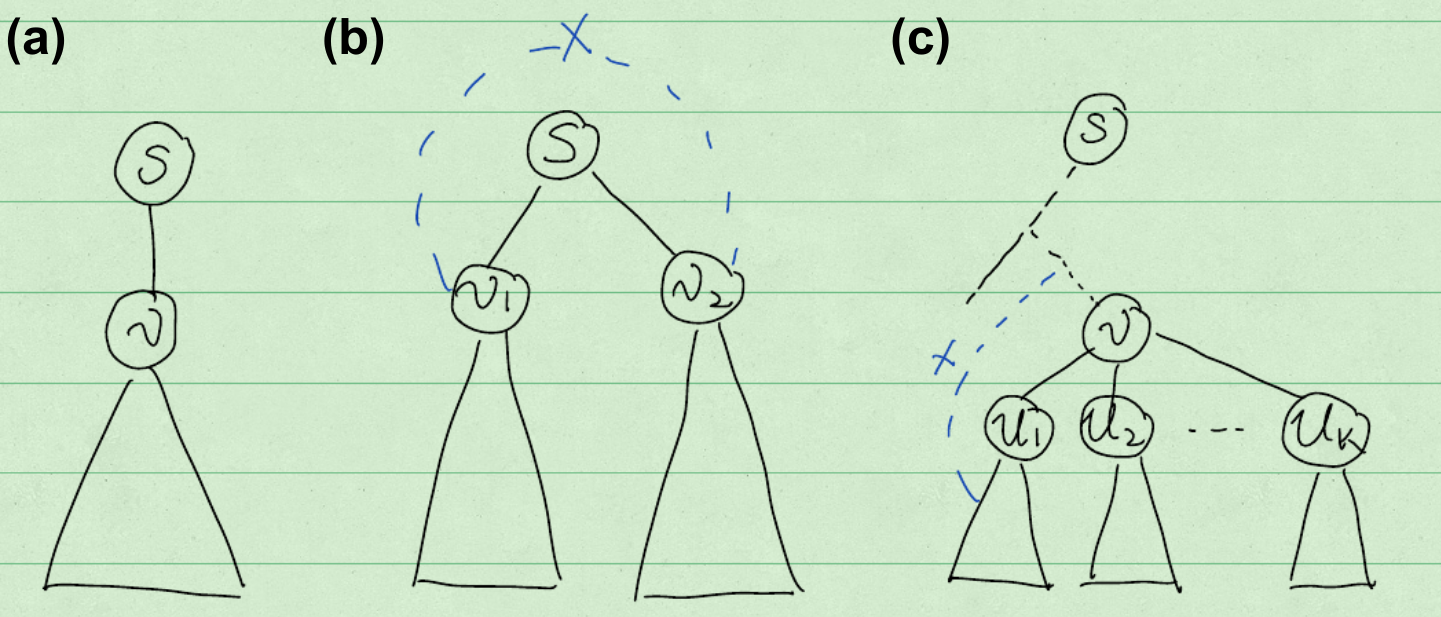
\includegraphics[width=0.8\textwidth]{find-articulation.png}
\end{figure}

\subsection{DFS: Find Bi-connected Components.}
\paragraph{Main idea:} Store visited edges in a stack while DFS on a graph and keep looking for Articulation Points. 
\begin{itemize}
 \item As soon as an Articulation Point $u$ is found, all edges visited while DFS from node $u$ onward will form one biconnected component. 
 \item When DFS completes for one connected component, all edges present in stack will form a biconnected component.
 \item If there is no Articulation Point in graph, then graph is biconnected and so there will be one biconnected component which is the graph itself.
\end{itemize}

\subsubsection{How to check articulation point?}
\begin{claim}
 If $u$ is an ancestor of $v$ in the DFS tree, then $s(u) < s(v)$.
\end{claim}
\paragraph{Note:} smaller number of start time $s$ means higher up of the tree. 

How the algorithm works? What does DFS keep track of? 

We want to know which vertices as we go back out of the subtree could be 
articulation points. The higher a back edge goes, the more vertices are ruled 
out to be articulation points. So \textbf{keep track of the highest back edge 
going out from every subtree}. Hence we are able to find the highest ancestor 
that an edge going through from the subtree. Then we know every vertex along the 
way can not be articulation point because of this subtree. (But still, other 
subtrees may cause them to be an articulation point.)

This is where the postorder comes in. In the example, suppose $x_1$ goes to vertex $p_1$ which is the highest back edge to reach from any where of $T(x_1)$. So the smallest number of start time reached from $T(x_1)$ is $s(p_1)$. From $x_2$ we have some edge goes up to vertex $p_2$, which is the highest back edge to reach from any where of $T(x_2)$.

\begin{figure}[H]
\centering
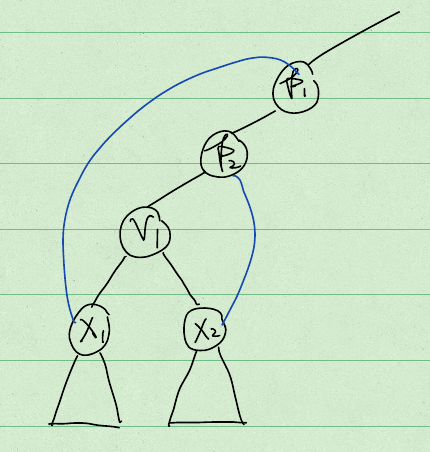
\includegraphics[width=0.3\textwidth]{dfs-claim.png}
\end{figure}

\begin{definition}
 \textbf{low(x)} is the smallest \textbf{start time} of vertices reachable by a back edge from subtree rooted at $x$. 
\end{definition}

Suppose $v$ has just two child $x_1$ and $x_2$,
\[\text{low}(v) = \min (\text{low}(x_1), ~\text{low}(x_2), ~\text{s}(u): (v, u) \text{ is a back edge})\]

What make $v$ an articulation point?
\begin{claim}
 For any node $v$ that is not the root, $v$ is an articulation point \textbf{if 
and only if }
 
 there exist a child $u_i$ of $v$ such that $\text{low}(u_i) \ge s(v)$.
\end{claim}

\paragraph{Notes:} The claim means the child of $v$ will not send any back edge 
to any where above $v$. Sending back edges only to $v$ and below means removing 
$v$ the whole subtree will fall apart.
\subsection{Wrapper of DFS}
DFS is used to search the entire graph. Usually DFS is wrapped by another 
function to traverse all the vertices in the graph.

DepthFirstSearch($G$):\\
\tab \tab While there is an unexplored vertex $x$,\\
\tab \tab \tab dfs($G$, $x$)

\subsubsection{Time}
In this case, we still have start time and finish time continue all the way 
though the outside layer. We start from inner layer of one $s$ and you might 
advance to certain point of time then find out that you have no more vertex to 
visit. So we go back to the outer loop start DFS at some other point and keep 
the time going. So the start time and finish will still between $1$ and $2n$.
\section{Directed Graph}
In directed graph, an edge is an ordered pair. 
\subsection{Edges}
\begin{itemize}
 \item Tree edges: edges where new vertices are discovered.
 \item Back edges: $(3 \rightarrow 1)$
 \item Forward edge $(1 \rightarrow 3)$ could be forward edge if DFS went $(1 
\rightarrow 2 \rightarrow 3)$.
 \item Cross edge
\end{itemize}

\begin{figure}[H]
\centering
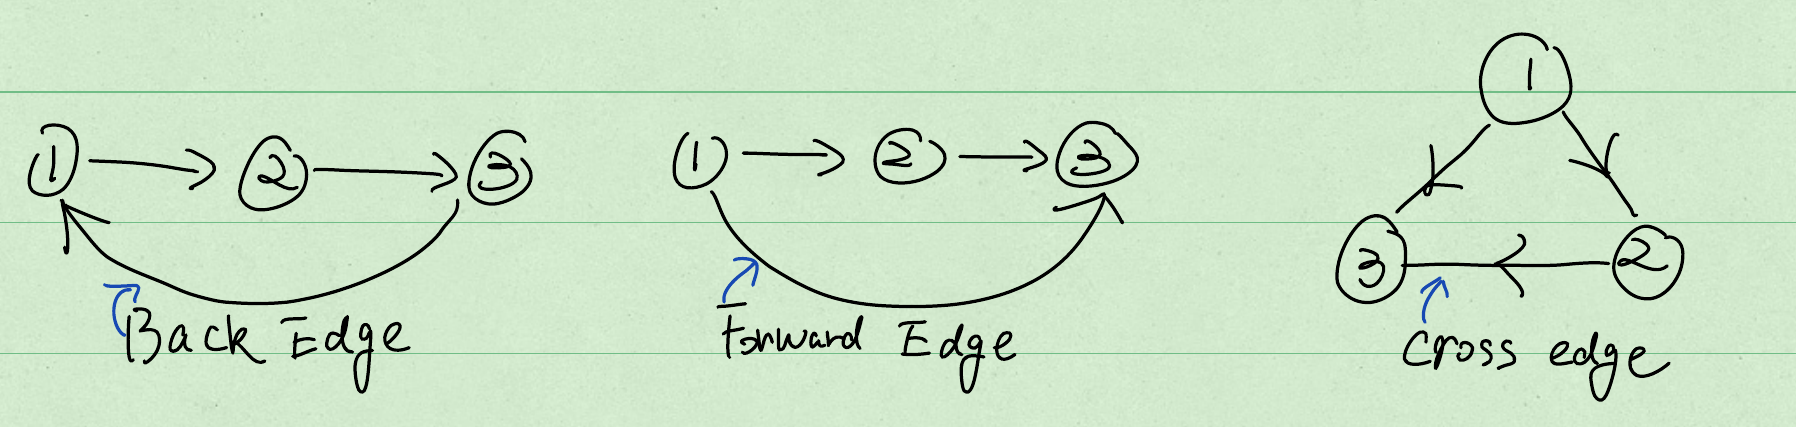
\includegraphics[width=0.45\textwidth]{edges.png}
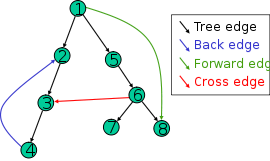
\includegraphics[width=0.3\textwidth]{edges-2.png}
\end{figure}
\begin{claim}
\textbf{Restriction of cross edge:} If $(u, v)$ is a cross edge, then 
$s(u)$ > $s(v)$. In other words, $v$ is discovered before $u$.
\end{claim}
\begin{claimproof}
By contradiction, if $(u, v)$ is a cross edge and $u$ is discovered before $v$, 
we cannot let DFS left $u$ and discover $v$ without go though $(u, v)$. 
Therefore, $v$ will be a child of $u$ instead of a node in other DFS tree.
\end{claimproof}
\subsection{Directed Acyclic Graph (DAG)}
\subsubsection{Maximum Number of edges}
\begin{itemize}
\item How many edges a undirected \textbf{acyclic} graph could have at most? 
$N-1$
\item How many edges a directed \textbf{acyclic} graph could have at most? 
$\frac{N(N-1)}{2}$
\end{itemize}
\subsubsection{Algorithm}
\begin{itemize}
 \item Input: Directed acyclic graph $G$.
 \item Goal: Solve topological sort problem by finding the topological order. 
In other words, find an order of the vertices such that for each edge $(u, v)$, 
$u$ precedes $v$ in order.
\end{itemize}
\begin{theorem}
 Any directed acyclic graph has a topological order.
\end{theorem}

\begin{proof}
Show every DAG has some node with no incoming edges. Then remove the node from 
the graph and get a smaller DAG. Then use induction to prove the theorem is 
true.

\begin{claim}
Every DAG has some node with no incoming edge.
\end{claim}
\begin{claimproof}
Given a graph DAG and reverse the directions of all the edges. Then we want to 
argue that there is no outgoing edge for some nodes in the graph.

For contradiction, suppose the argument is not true and every node has some 
outgoing edge. Then start walking from some vertex $v$ and this walking will 
keep on continuing since every vertex has some outgoing edge. But the graph is 
finite. Continuing walking on a finite graph means there must be cycles in the 
graph. We meet a contradiction since the graph is DAG.
\end{claimproof}
\end{proof}

The first principle algorithm for topological sorting is to track the in-degree 
of every vertex, which is the number of edges come in to the vertex. First 
output the vertex $v$ with in-degree zero. Then go to the adjacency list of $v$ and decrease the in-degree of every neighbor by 1. Remove $v$ from the graph and 
repeat.

Solution based DFS.
\begin{theorem}
 If $G$ is a DAG and $(u, v)$ is an edge, then on any DepthFirstSearch($G$), 
$f(u) \ge f(v)$.
\end{theorem}

\begin{proof}
Prove by cases analysis.
 \begin{itemize}
  \item Case 1: $s(u) < s(v)$. $u$ is discovered before $v$. Then $v$ will 
become a descendant of $u$ (may not be child).
  \item Case 2: $s(u) > s(v)$. $v$ is discovered before $u$. 
  \begin{itemize}
   \item If we discovered $u$ in the course of DFS($v$), then there must be 
a path from $v$ to $u$, which means $G$ has a cycle. 
$\Rightarrow\mskip-\thinmuskip\Leftarrow$
    \item If $u$ is not in the subtree of $v$ as the following example, 
then obviously $f(v) < f(u)$.
        \begin{figure}[H]
        \centering
        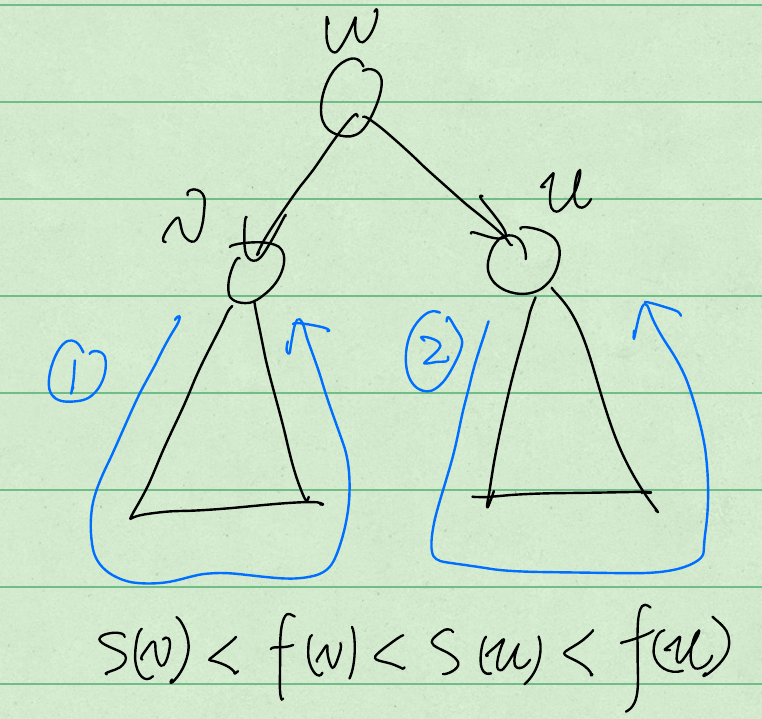
\includegraphics[width=0.3\textwidth]{dfs-s-f.png}
        \end{figure}
  \end{itemize}
 \end{itemize}
\end{proof}

So, \[s(v) < f(v) < s(u) < f(u)\]
Therefore the algorithm should be:

TopologicalSort($G$):\\
\tab\tab DepthFirstSearch($G$):\\
\tab\tab\tab\tab Output vertices in reverse order of finish time.

\subsection{Strongly Connected Graph}

\subsubsection{Basics}
Give a directed graph $G = (V, E)$, what is the correct connectivity relation?

We want the relation to be equivalent. The edge between two nodes is not 
symmetric relation in directed graph. Therefore we create a equivalent relation 
by setting symmetric in the definition.

\begin{definition}
 $R = \{(u, v): \text{There are paths from $u$ to $v$ and from $v$ to $u$}\}$
\end{definition}

$R$ is reflective, symmetric and transitive. So $R$ is an equivalent relation 
on the vertices.

\begin{definition}
$R$ partitions $V$ onto $V_1,~V_2,~\cdots, V_k$. (Equivalence Classes)

If $V_1 \subset V$, which is the vertex set of $G = (V, E)$, it induces the 
sub-graphs
\[G_{V_i} = (V_i, ~E \cap (V_i \times V_i) )\]
For simplicity, call $G_{V_i}$ as $G_i$. $G_i$'s are \textbf{the 
strongly connected components} of $G$.
\end{definition}


It is possible to have edges connecting different strongly connected 
components. See example as follows.
\begin{figure}[H]
\centering
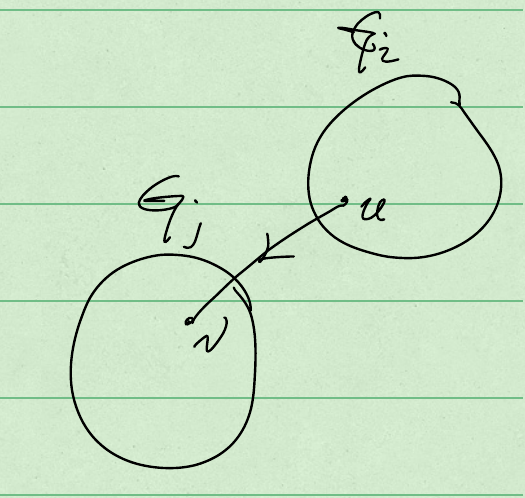
\includegraphics[width=0.2\textwidth]{edge-strongly-connected-components.png}
\end{figure}

\begin{definition}
 The \textbf{strongly connected graph} of directed graph $G(V, E)$ is 
$G_{SCC}(V_{SCC}, E_{SCC})$, where
\begin{itemize}
 \item $V_{SCC} = \{c_i: G_i \text{ is a strongly connected components}\}$.
 \item $E_{SCC} = \{(c_i, c_j): \exists v_i \in G_i \text{ and }v_j \in G_j, 
~(v_i, v_j) \in E \}$
\end{itemize}
\end{definition}
Here $G_{SCC}$ is actually a quotient graph.

Example, $(a)$ in the following plot is the Graph $G$ and $(b)$ is the strongly 
connected graph of $G$. The equivalence class of $G$ is $\{\{1, 2, 3, 4\}, 
\{3, 6, 7\}\}$.

\begin{figure}[H]
\centering
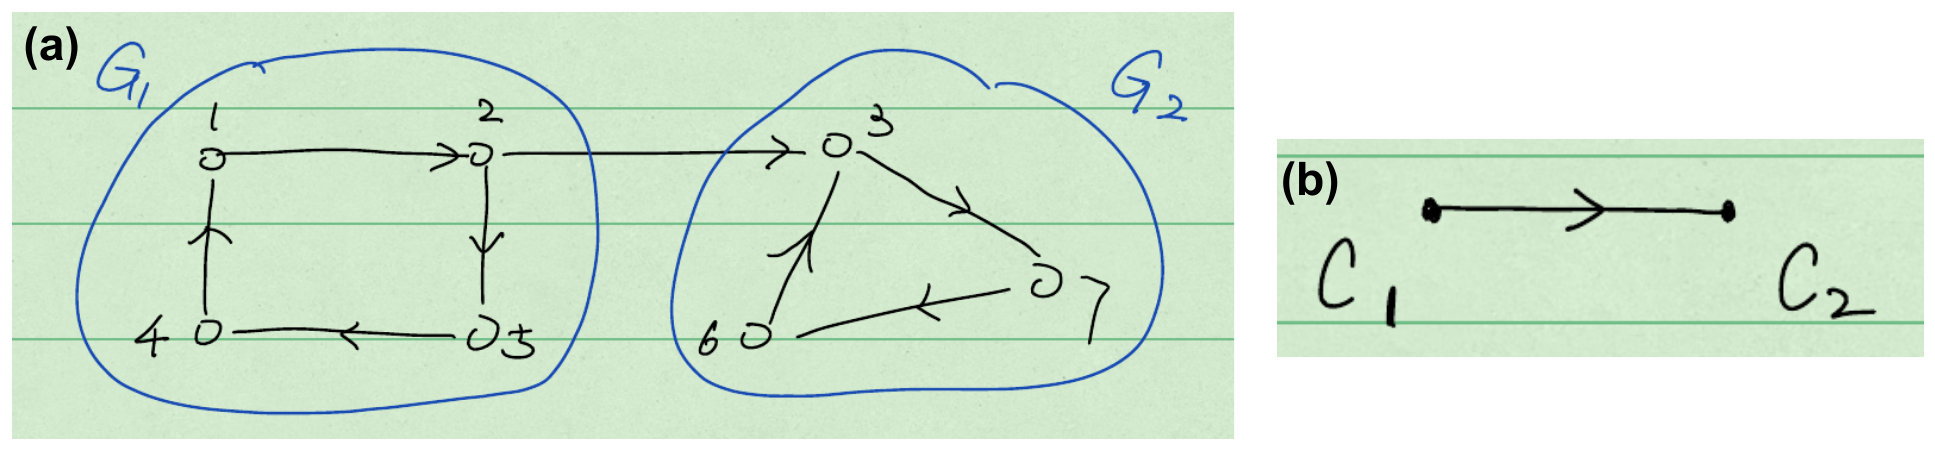
\includegraphics[width=0.7\textwidth]{scg.png}
\end{figure}

\begin{theorem}
 $G_{SCC}$ is acyclic.
\end{theorem}

\begin{proof}
 The components we have found are the maximal with respect to the relation on 
both side to reach other. Prove the theorem by contradiction. Suppose we have a 
cycle as the following plot. Because there must be a path from $u$ to $v$ and 
vice versa. Then , we are able to merging $G_1$, $G_3$. In fact, all three 
components can be merged together.

\begin{figure}[H]
\centering
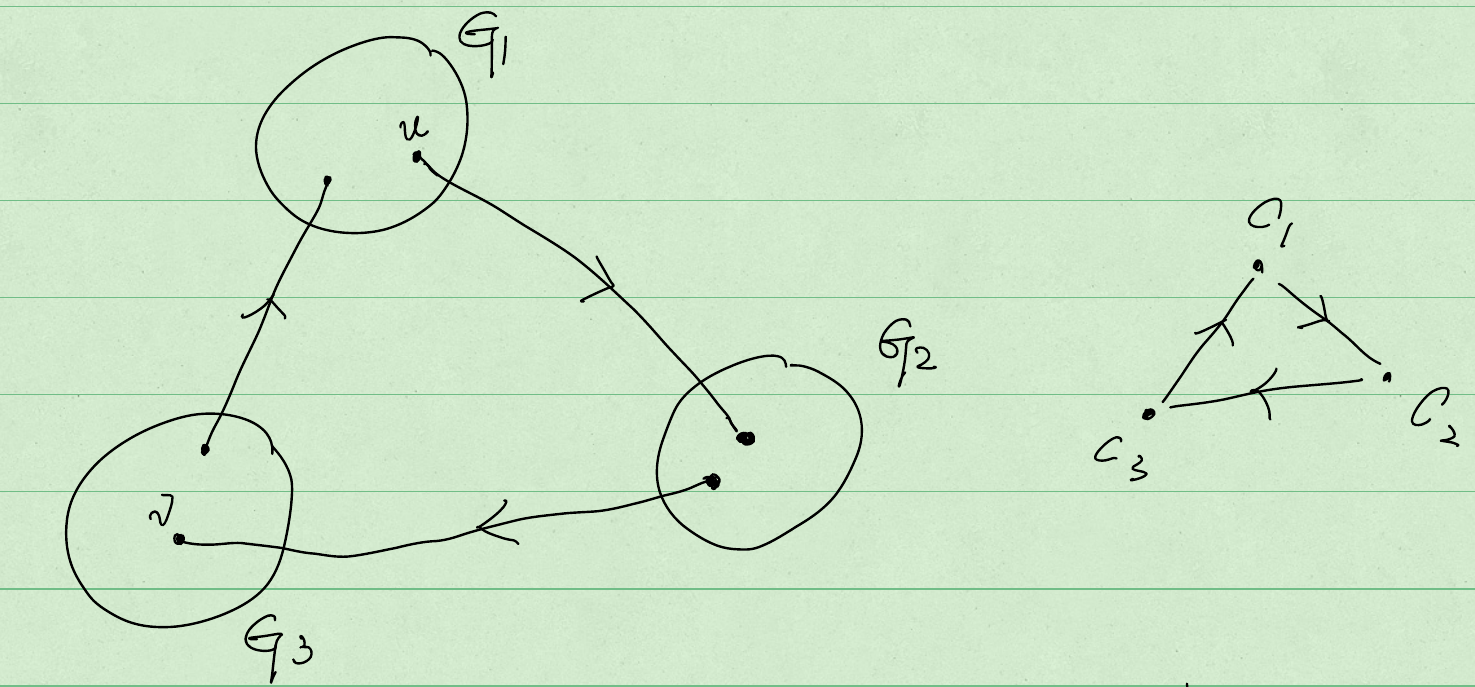
\includegraphics[width=0.45\textwidth]{scg-contradiction.png}
\end{figure}
\end{proof}

Many algorithm on directed graph works on first decomposing the graph into 
strongly connected components.

DFS decomposes a directed graph into SCC's.

\subsubsection{Finish Time}
Now we first gave a \textbf{false theorem} and make it right.
\begin{theorem}\textbf{[False Theorem]}

Suppose $G$ is an arbitrary graph and $G_{SCC}$ is a DAG. If $c_i, ~c_2 \in V_{SCC}$ are nodes corresponding to two SCC's $G_1$ and $G_2$ in $G$ and $(c_i, ~c_2) \in E_{SCC}$, then in DFS($G$), every vertex in $G_1$ finish after every vertex in $G_2$. 
\end{theorem}

\begin{proof}
 Prove the theorem is false by a counter example as follows:
\begin{figure}[H]
\centering
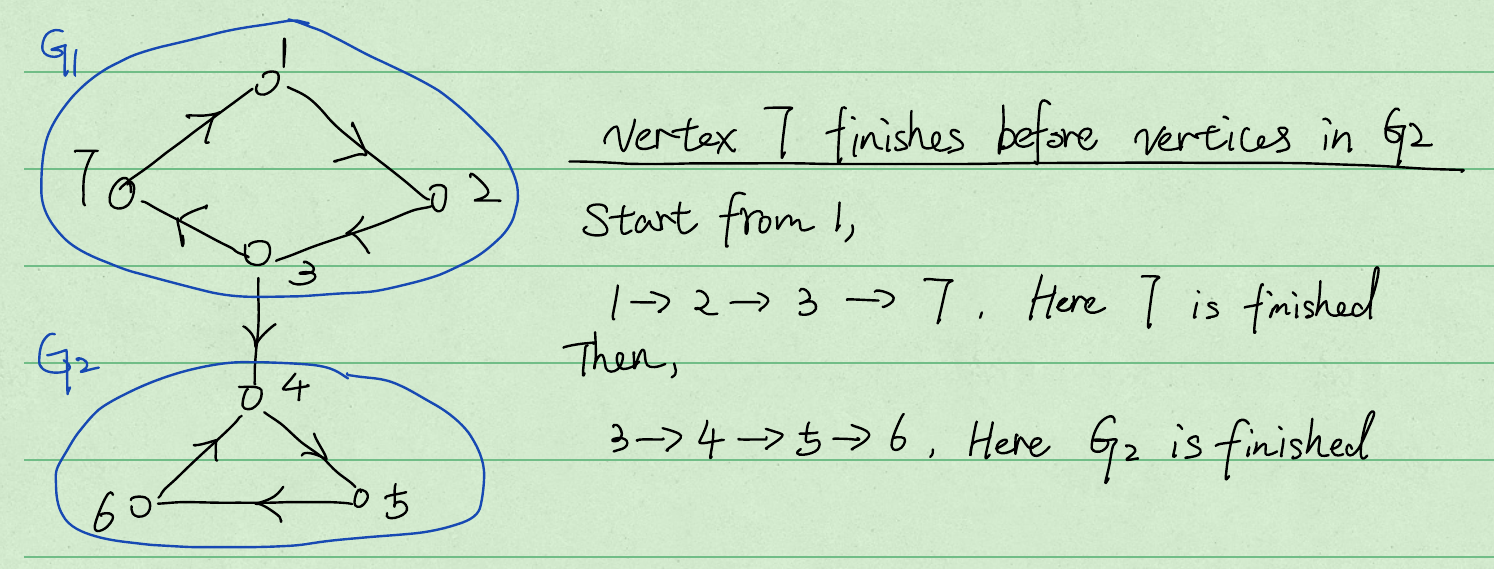
\includegraphics[width=0.7\textwidth]{scc-finish-time.png}
\end{figure}
\end{proof}

\begin{theorem}\textbf{[Updated Theorem]}

Suppose $G$ is an arbitrary graph and $G_{SCC}$ is a DAG. If $c_i, ~c_2 \in V_{SCC}$ are nodes corresponding to two SCC's $G_1$ and $G_2$ in $G$ and $(c_i, ~c_2) \in E_{SCC}$, then in DFS($G$), \textbf{there exist a vertex} in $G_1$ finish after every vertex in $G_2$. 
\end{theorem}

\begin{proof}
 TODO: Read the proof in the book.
\end{proof}

\subsubsection{Kosaraju's Algorithm}
\begin{definition}
$G_{SCC}$ is a DAG. So, $G_{SCC}$ has one or more vertices with no in-coming 
edges. These vertices are called \textbf{sources}.
\end{definition}

\begin{claim}{}
If $v$ is the vertex with largest $f(v)$ in a DFS($G$). Then $v$ must lies in 
the source component. 
\end{claim}

\begin{claimproof}{}
Prove by contradiction.

If $v$ does not lie in the source component but in some other component $C$. So 
$v$ must have some in-coming edge to make it not a source. That means that 
some vertex $u$ must finish later than everything in the component $C$ because 
of the theorem of finishing time. Therefore $v$ could not be the latest 
finishing vertex.
\begin{figure}[H]
\centering
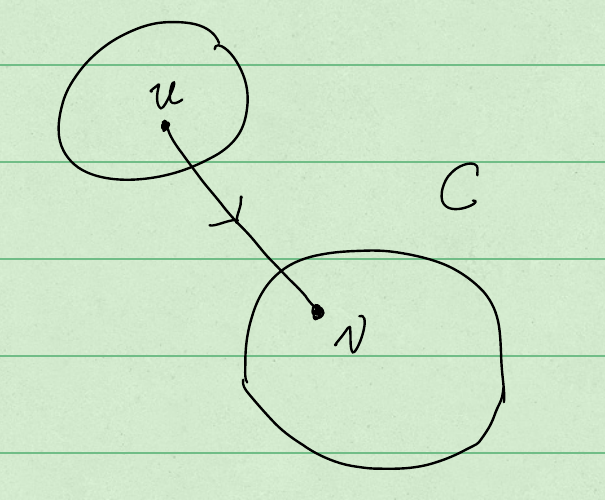
\includegraphics[width=0.3\textwidth]{source-finish-time.png}
\end{figure}
\end{claimproof}


\paragraph{Kosaraju Algorithm}
\begin{itemize}
 \item One DFS(G) to record the nodes of finish times. Let $f_1(v)$ be the 
finish time of $v$ in this DFS.
\item Reverse all the edges in $G$ to create the graph $G^R$.
\item Do DFS($G^R$) with one constrain:
    \begin{itemize}
    \item In the outer procedure, always choose the undiscovered vertex $v$ 
with the greatest $f(v)$.
    \end{itemize}
\end{itemize}

\paragraph{Notes}
\begin{itemize}
 \item The vertex $v$ with greatest $f_1(v)$ lies in a sink component of $G^R$.
\item $G$ and $G^R$ have the same strongest connected component DFS($G^R$) start 
at $v$ will only discover the SCC containing $v$.
\item When the inner call to DFS($G^R, ~v$) finishes, output all the discovered 
vertices as one SCC of $G$.
\item When we return to the outer loop and pick the undiscovered vertex with 
the greatest finish time, we know inductively that we will find all SCC's.
\end{itemize}

\begin{figure}[H]
\centering
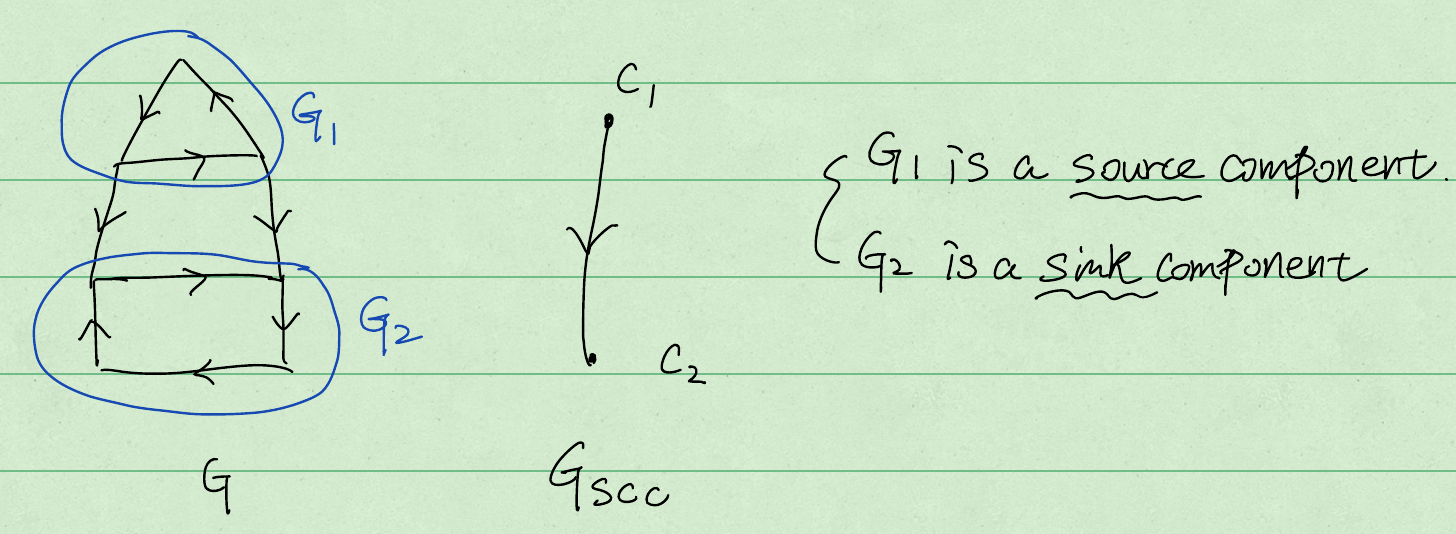
\includegraphics[width=0.6\textwidth]{scc-source-sink.png}
\end{figure}

\paragraph{Running Time}
Two DFS's and reverse the edges in the graph. All the steps are linear. So 
this is a $O(m + n)$ algorithm. $m, n$ are the numbers of vertices and edges.